\documentclass[12pt]{exam}
\usepackage{amsmath, amssymb}
\usepackage{booktabs, tabularx} % For text alignment on cover page
\usepackage{epsfig}             % For \includegraphics command

\newcolumntype{C}{>{\centering\arraybackslash}X}

\begin{document}
\addpoints
\setlength{\parindent}{0cm}

\begin{center}

{\Large\textbf{MATH 040 - Final Exam Preview}}\\
\medskip
{\Large{Spring 2020}}

\vskip1cm
\makebox[0.7\textwidth]{\large Last Name:\enspace\hrulefill}
\vskip0.4cm
\makebox[0.7\textwidth]{\large First Name:\enspace\hrulefill}
\vskip0.4cm

\makebox[0.7\textwidth]{\large Signature:\enspace\hrulefill}
\vskip0.4cm

\end{center}
\bigskip
\textbf{Instructions:}
\begin{itemize}
  \item Try to complete the entire exam, but know that you're welcome to stop after 2 hours--even if the exam is not completed. Please record how much time
  you spent on this front page.
  \item Some subset of the questions on this Final Exam Preview will be selected (and perhaps slightly modified) together with some questions from the quizzes and Midterm Preview to make up your Final Exam.
  \item This Final Exam Preview is longer than the actual final exam, so
  don't worry if you don't complete the whole thing in under an hour.
  \item This Preview will be graded as participation only! I will let everyone
  know which problems they got right or wrong, but everyone who completes the
  assignment will receive full credit.
  \item Feel free to use calculators, books, the internet, your instructors, and
  any TAs or tutors. However, books, the internet, and instructors will not be
  available when you take the actual Final Exam.
  \item If anything is unclear, please give feedback by writing your remark next to the question.
  \item Please show as much work as possible, because that allows me to give you the best feedback.
\end{itemize}
\vskip0.4cm
\makebox[0.7\textwidth]{\large Time Spent:\enspace\hrulefill}
\vskip0.4cm
\begin{center}
  \gradetable[h][questions]
\end{center}

\newpage
\vskip1cm

%
\begin{questions}
\pagebreak

\question[5] {
  Simplify the expressions as much as possible. \begin{parts}
    \item $\displaystyle 6^{-2}\cdot3^3$
    \item $\displaystyle 5^{3/2} \cdot \sqrt{5}$
    \item $\displaystyle \sqrt{50} + \sqrt{32} + \sqrt{18}$
    \item $\displaystyle 6^0$
    \item $\displaystyle (2^{3/4})^2$
  \end{parts}
}

\question[5] {
  Evaluate the following expressions \begin{parts}
    \item $3^a + 2^a$ when $a = -2$
    \item $(b^2 + c)^{1/2}$ when $b = -3$ and $c = 7$
    \item $\displaystyle 3d\left(\frac{d^2}{d^{-1}}\right)^2$ when $d = 10$
    \item $\displaystyle \left(\frac{1}{x}\right)^{-3}$ when $x = 7^2$ \hspace{1cm} \textit{(Write in the form $a^b$.)}
  \end{parts}
}
\pagebreak

\question[10] {
  Right now the UN approximates that roughly $800\,000\,000$ people in the
  world lack the necessary food to live a healthy lifestyle. The UN also
  estimates ending world hunger each year would cost about $\$30\,000\,000\,000$
  per year. In 2019, the US defense budget was approximately $\$700$ billion.
  \begin{parts}
    \part Write $800\,000\,000$ in scientific notation.
    \part Write $\$30\,000\,000\,000$ in scientific notation.
    \part Write $\$700$ billion in scientific notation.
    \part Ending world hunger would cost what percentage of the annual US defense budget?
    \part How much does the UN Estimate it would cost on a \textit{per person} per year basis to end world hunger?
  \end{parts}
}
\pagebreak
\question[6] {
  Escape velocity is the minimum speed an object must reach to escape the pull of a planet's gravity (ignoring wind resistance).
  The escape velocity from planet earth is $v$ where \[
    v = \sqrt{\frac{2Gm}r}
  \] where \begin{alignat*}{2}
   G &= 6.5 \times 10^{-11}\ \text{m}^3/(\text{kg}\cdot \text{s}^2)
    &&\hspace{2cm} \text{(universal gravitational constant)} \\
   m &= 6.0 \times 10^{24}\ \text{kg}
    &&\hspace{2cm} \text{(mass of earth)} \\
   r &= 6.5 \times 10^6\ \text{m}
    &&\hspace{2cm} \text{(radius of earth)}
  \end{alignat*}
  \begin{parts}
    \part What is the escape velocity from earth in meters per second?
    \\ \vspace{8cm}
    \part Using the information that one mile is 1.6 kilometers, what is the escape velocity in miles per hour?
  \end{parts}
}
\pagebreak
\question[10] {
  Given a square based pyramid with equilateral triangles for faces and side length $\ell$, the height, surface area, and volume is given by \begin{alignat*}{2}
   h &= \frac{\sqrt{2}}{2}\ell      &&\hspace{2cm} \text{(height)} \\
   A &= (1 + \sqrt{3})\ell^2        &&\hspace{2cm} \text{(surface area)} \\
   V &= \frac{\sqrt 2}6\ell^3       &&\hspace{2cm} \text{(volume)}
  \end{alignat*}
  If the volume of the Great Pyramid of Giza is $2\,600\,000\ \text{m}^3$, what is its height?
}
\pagebreak
\question[10] {
  % Use Heron's formula to find area?
  The distance between two points $(x_1, y_1)$ and $(x_2, y_2)$ is given by \[
    d = \sqrt{(x_2 - x_1)^2 + (y_2 - y_1)^2}.
  \]
  Consider the triangle with vertices $(1,-2)$, $(6,3)$, and $(7,-4)$.
  \begin{parts}
    \part Draw the triangle.\\
    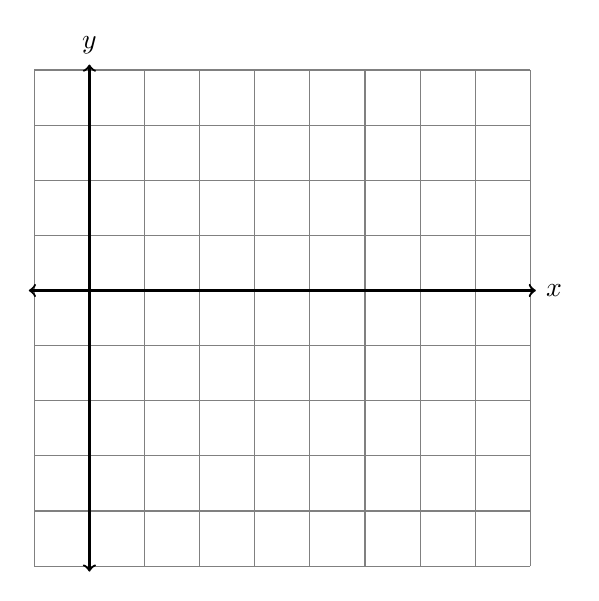
\begin{tikzpicture}[scale=0.7]
      \draw[gray] (-1,-5) grid (8, 4);
      \draw[thick,<->] (-1.1,0)--(8.1,0) node[right] {$x$};
      \draw[thick,<->] (0,-5.1)--(0,4.1) node[above] {$y$};
    \end{tikzpicture}
    \part What is the length of the longest side? (Simplify the radical as much as possible.)
    \part What is the length of the shortest side?
    \part What is the perimeter of the triangle?
    \part Is this an equilateral triangle, an isosceles triangle, or a scalene triangle?
  \end{parts}
}
\pagebreak
\question[10] {
  One way to create a box (with no top) is to take a rectangular piece of
  cardboard, cut squares from each of the corners, and fold up the sides.
  Suppose you start with a piece of cardboard of width $w$ and length $\ell$ and
  cut out corners of size $h$, as shown below in the diagram, where the dashed
  region is the base of the box.\\~\\
  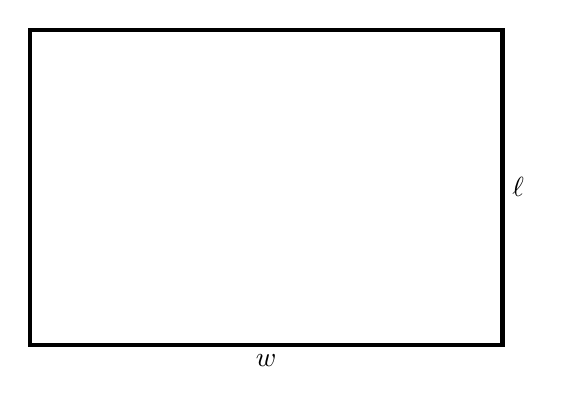
\begin{tikzpicture}
    \draw[ultra thick] (0,0) rectangle (6,4);
    \node at (6.2,2) {$\ell$};
    \node at (3,-0.2) {$w$};
  \end{tikzpicture}\hspace{2cm}
  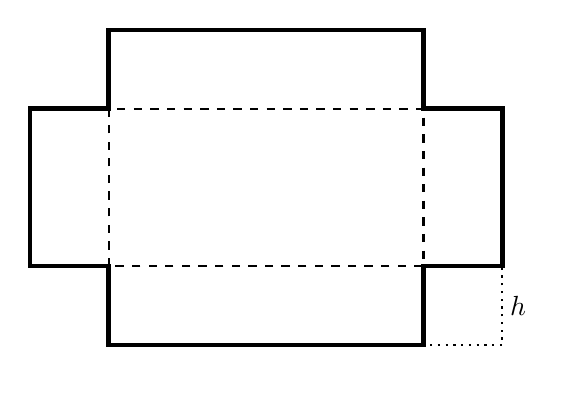
\begin{tikzpicture}
    \draw[ultra thick] (0,1)--(0,3)--(1,3)--(1,4)--(5,4)--(5,3)--(6,3)--(6,1)--(5,1)--(5,0)--(1,0)--(1,1)--cycle;
    \draw[dashed, thick] (1,1) rectangle (5,3);
    \draw[dotted, thick] (5,1) rectangle (6,0);
    \node at (6.2,0.5) {$h$};
    \node at (3,-0.2) {$ $};
  \end{tikzpicture}
  \begin{parts}
    \part What is the height of the box?
    \part What are the dimensions of the base of the resulting box?
    \part What is the surface area of the box?
    \part What is the volume of the box in terms of $w, h,$ and $\ell$?
    \part What is the volume of the box specifically when $w = 9$, $h = 2$, and $\ell = 8$?
  \end{parts}
}
\pagebreak
\question[10] {
  Consider the polynomial $p(x) = -x^3 + x^2 + 2x$.
  \begin{parts}
    \part Factor $p(x)$.
    \part What are its roots?
    \part Determine
      $\displaystyle \lim_{x \rightarrow \infty} p(x)$ and
      $\displaystyle \lim_{x \rightarrow -\infty} p(x)$.
    \part Graph $p(x)$ including its roots and end behavior.

    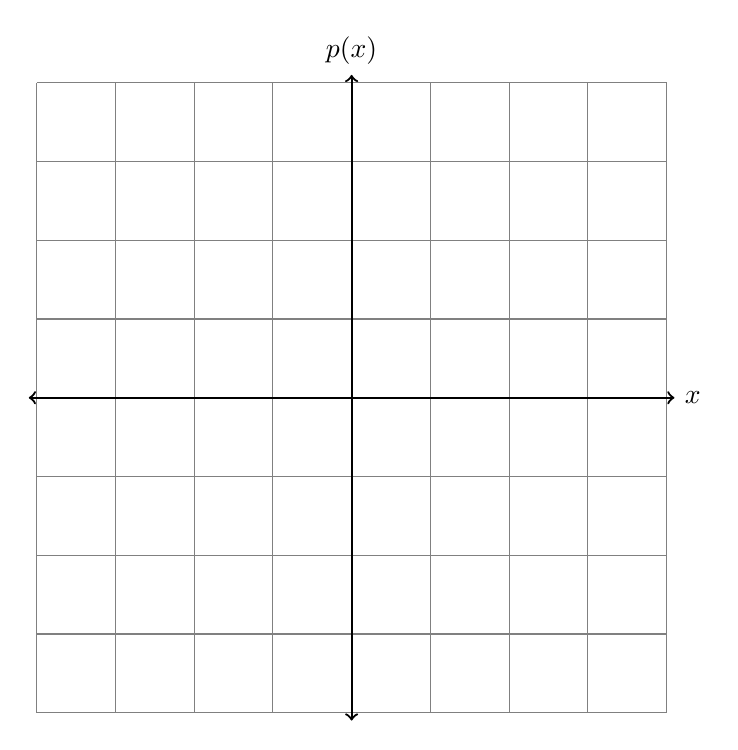
\begin{tikzpicture}
      \draw[gray] (-4,-4) grid (4, 4);
      \draw[thick,<->] (-4.1,0)--(4.1,0) node[right] {$x$};
      \draw[thick,<->] (0,-4.1)--(0,4.1) node[above] {$p(x)$};
    \end{tikzpicture}
    \part What is the domain and range of $p(x)$? \\~\\~\\
  \end{parts}
}
\pagebreak
\question[5] {
    % At Rogelio's restaurant, \textit{Los Muchachos Nachos}, there are three choices of chips, four choices of cheese, five choices of salsa, and eight additional toppings (e.g. jalape\~nos, olives, sour cream) that you can either put on or leave off.
    % \\
    % The nachos must include exactly one kind of chip, one kind of cheese, and one kind of salsa.
    % How many different nacho platters are possible to make?
  %   \\ \vspace{4cm}
    % Suppose that Olivia can paint a fence in four hours and Keenan can paint a
    % fence in five hours. How long does it take Olivia and Keenan to paint a
    % fence together?
  %   \\ \vspace{6cm}
  %   \part
    Jessica swims at $2$ miles per hour in a swimming pool (which has no current).
    When she swims in a river with a slight current, it takes her $50\%$ longer
    to swim upstream from Dock A to Dock B than it takes for her to swim
    downstream from Dock B to Dock A.
    Using this information, what is the speed of the current in the river?
  % \end{parts}
}
\pagebreak
\question[15] {
  The position of a basketball thrown from a height of six feet at a speed of $v$ feet per second upward is given by \[
    h_v(t) = -16t^2 + vt + 6
  \]
  where $h_v(t)$ is the height of the ball $t$ seconds after the ball is thrown.
  \begin{parts}
    \part Use the quadratic equation to find the roots of $h_v$ where $v$ is a variable.
    \textbf{For the remaining questions, assume $v = 20$, so that $h(t) = -16t^2 + 20t + 6$.}
    \part What is the value of $t$ at which the ball hits the ground?
    \part If the ball is at its highest point at the \textit{average} of its two
    roots, what is the value of $t$ at which the ball attains its maximum height?
    How high is it?
    \\\textit{(Hint: one of the roots should be negative.)}
    \part Suppose the ball is a basketball being shot up to a 10 foot rim.
    At what value of $t$ does the basketball go through the basket?
    \\\textit{(Hint: The time should be \textbf{after} the time found in part (c).)}
  \end{parts}
}
\end{questions}
\end{document}
